\documentclass[]{article}
\usepackage{lmodern}
\usepackage{amssymb,amsmath}
\usepackage{ifxetex,ifluatex}
\usepackage{fixltx2e} % provides \textsubscript
\ifnum 0\ifxetex 1\fi\ifluatex 1\fi=0 % if pdftex
  \usepackage[T1]{fontenc}
  \usepackage[utf8]{inputenc}
\else % if luatex or xelatex
  \ifxetex
    \usepackage{mathspec}
  \else
    \usepackage{fontspec}
  \fi
  \defaultfontfeatures{Ligatures=TeX,Scale=MatchLowercase}
\fi
% use upquote if available, for straight quotes in verbatim environments
\IfFileExists{upquote.sty}{\usepackage{upquote}}{}
% use microtype if available
\IfFileExists{microtype.sty}{%
\usepackage{microtype}
\UseMicrotypeSet[protrusion]{basicmath} % disable protrusion for tt fonts
}{}
\usepackage[margin=1in]{geometry}
\usepackage{hyperref}
\hypersetup{unicode=true,
            pdftitle={Solutions to Recommended Exercises},
            pdfauthor={Thea Roksvåg, Ingeborg Hem and Mette Langaas, Department of Mathematical Sciences, NTNU},
            pdfborder={0 0 0},
            breaklinks=true}
\urlstyle{same}  % don't use monospace font for urls
\usepackage{color}
\usepackage{fancyvrb}
\newcommand{\VerbBar}{|}
\newcommand{\VERB}{\Verb[commandchars=\\\{\}]}
\DefineVerbatimEnvironment{Highlighting}{Verbatim}{commandchars=\\\{\}}
% Add ',fontsize=\small' for more characters per line
\usepackage{framed}
\definecolor{shadecolor}{RGB}{248,248,248}
\newenvironment{Shaded}{\begin{snugshade}}{\end{snugshade}}
\newcommand{\KeywordTok}[1]{\textcolor[rgb]{0.13,0.29,0.53}{\textbf{#1}}}
\newcommand{\DataTypeTok}[1]{\textcolor[rgb]{0.13,0.29,0.53}{#1}}
\newcommand{\DecValTok}[1]{\textcolor[rgb]{0.00,0.00,0.81}{#1}}
\newcommand{\BaseNTok}[1]{\textcolor[rgb]{0.00,0.00,0.81}{#1}}
\newcommand{\FloatTok}[1]{\textcolor[rgb]{0.00,0.00,0.81}{#1}}
\newcommand{\ConstantTok}[1]{\textcolor[rgb]{0.00,0.00,0.00}{#1}}
\newcommand{\CharTok}[1]{\textcolor[rgb]{0.31,0.60,0.02}{#1}}
\newcommand{\SpecialCharTok}[1]{\textcolor[rgb]{0.00,0.00,0.00}{#1}}
\newcommand{\StringTok}[1]{\textcolor[rgb]{0.31,0.60,0.02}{#1}}
\newcommand{\VerbatimStringTok}[1]{\textcolor[rgb]{0.31,0.60,0.02}{#1}}
\newcommand{\SpecialStringTok}[1]{\textcolor[rgb]{0.31,0.60,0.02}{#1}}
\newcommand{\ImportTok}[1]{#1}
\newcommand{\CommentTok}[1]{\textcolor[rgb]{0.56,0.35,0.01}{\textit{#1}}}
\newcommand{\DocumentationTok}[1]{\textcolor[rgb]{0.56,0.35,0.01}{\textbf{\textit{#1}}}}
\newcommand{\AnnotationTok}[1]{\textcolor[rgb]{0.56,0.35,0.01}{\textbf{\textit{#1}}}}
\newcommand{\CommentVarTok}[1]{\textcolor[rgb]{0.56,0.35,0.01}{\textbf{\textit{#1}}}}
\newcommand{\OtherTok}[1]{\textcolor[rgb]{0.56,0.35,0.01}{#1}}
\newcommand{\FunctionTok}[1]{\textcolor[rgb]{0.00,0.00,0.00}{#1}}
\newcommand{\VariableTok}[1]{\textcolor[rgb]{0.00,0.00,0.00}{#1}}
\newcommand{\ControlFlowTok}[1]{\textcolor[rgb]{0.13,0.29,0.53}{\textbf{#1}}}
\newcommand{\OperatorTok}[1]{\textcolor[rgb]{0.81,0.36,0.00}{\textbf{#1}}}
\newcommand{\BuiltInTok}[1]{#1}
\newcommand{\ExtensionTok}[1]{#1}
\newcommand{\PreprocessorTok}[1]{\textcolor[rgb]{0.56,0.35,0.01}{\textit{#1}}}
\newcommand{\AttributeTok}[1]{\textcolor[rgb]{0.77,0.63,0.00}{#1}}
\newcommand{\RegionMarkerTok}[1]{#1}
\newcommand{\InformationTok}[1]{\textcolor[rgb]{0.56,0.35,0.01}{\textbf{\textit{#1}}}}
\newcommand{\WarningTok}[1]{\textcolor[rgb]{0.56,0.35,0.01}{\textbf{\textit{#1}}}}
\newcommand{\AlertTok}[1]{\textcolor[rgb]{0.94,0.16,0.16}{#1}}
\newcommand{\ErrorTok}[1]{\textcolor[rgb]{0.64,0.00,0.00}{\textbf{#1}}}
\newcommand{\NormalTok}[1]{#1}
\usepackage{graphicx,grffile}
\makeatletter
\def\maxwidth{\ifdim\Gin@nat@width>\linewidth\linewidth\else\Gin@nat@width\fi}
\def\maxheight{\ifdim\Gin@nat@height>\textheight\textheight\else\Gin@nat@height\fi}
\makeatother
% Scale images if necessary, so that they will not overflow the page
% margins by default, and it is still possible to overwrite the defaults
% using explicit options in \includegraphics[width, height, ...]{}
\setkeys{Gin}{width=\maxwidth,height=\maxheight,keepaspectratio}
\IfFileExists{parskip.sty}{%
\usepackage{parskip}
}{% else
\setlength{\parindent}{0pt}
\setlength{\parskip}{6pt plus 2pt minus 1pt}
}
\setlength{\emergencystretch}{3em}  % prevent overfull lines
\providecommand{\tightlist}{%
  \setlength{\itemsep}{0pt}\setlength{\parskip}{0pt}}
\setcounter{secnumdepth}{0}
% Redefines (sub)paragraphs to behave more like sections
\ifx\paragraph\undefined\else
\let\oldparagraph\paragraph
\renewcommand{\paragraph}[1]{\oldparagraph{#1}\mbox{}}
\fi
\ifx\subparagraph\undefined\else
\let\oldsubparagraph\subparagraph
\renewcommand{\subparagraph}[1]{\oldsubparagraph{#1}\mbox{}}
\fi

%%% Use protect on footnotes to avoid problems with footnotes in titles
\let\rmarkdownfootnote\footnote%
\def\footnote{\protect\rmarkdownfootnote}

%%% Change title format to be more compact
\usepackage{titling}

% Create subtitle command for use in maketitle
\newcommand{\subtitle}[1]{
  \posttitle{
    \begin{center}\large#1\end{center}
    }
}

\setlength{\droptitle}{-2em}

  \title{Solutions to Recommended Exercises}
    \pretitle{\vspace{\droptitle}\centering\huge}
  \posttitle{\par}
  \subtitle{TMA4268 Statistical Learning V2019. Module 3: LINEAR REGRESSION}
  \author{Thea Roksvåg, Ingeborg Hem and Mette Langaas, Department of Mathematical
Sciences, NTNU}
    \preauthor{\centering\large\emph}
  \postauthor{\par}
      \predate{\centering\large\emph}
  \postdate{\par}
    \date{week 4 2019}


\begin{document}
\maketitle

{
\setcounter{tocdepth}{2}
\tableofcontents
}
Last changes: (18.01.2019: first version)

\section{Problem 1}\label{problem-1}

The Framingham Heart Study is a study of the etiology (i.e.~underlying
causes) of cardiovascular disease, with participants from the community
of Framingham in Massachusetts, USA. For more more information about the
Framingham Heart Study visit
\url{https://www.framinghamheartstudy.org/}. The dataset used in here is
subset of a teaching version of the Framingham data, used with
permission from the Framingham Heart Study.

We will focus on modelling systolic blood pressure using data from n =
2600 persons. For each person in the data set we have measurements of
the seven variables

\begin{itemize}
\tightlist
\item
  \texttt{SYSBP} systolic blood pressure,
\item
  \texttt{SEX} 1=male, 2=female,
\item
  \texttt{AGE} age in years at examination,
\item
  \texttt{CURSMOKE} current cigarette smoking at examination: 0=not
  current smoker, 1= current smoker,
\item
  \texttt{BMI} body mass index,
\item
  \texttt{TOTCHOL} serum total cholesterol, and
\item
  \texttt{BPMEDS} use of anti-hypertensive medication at examination:
  0=not currently using, 1=currently using.
\end{itemize}

A multiple normal linear regression model was fitted to the data set
with \texttt{-1/sqrt(SYSBP)} as response and all the other variables as
covariates.

\begin{Shaded}
\begin{Highlighting}[]
\KeywordTok{library}\NormalTok{(ggplot2)}
\CommentTok{#data = read.table("https://www.math.ntnu.no/emner/TMA4268/2018v/data/SYSBPreg3uid.txt")}
\NormalTok{data =}\StringTok{ }\KeywordTok{read.table}\NormalTok{(}\StringTok{"~/WWWemner/TMA4268/2018v/data/SYSBPreg3uid.txt"}\NormalTok{)}
\KeywordTok{dim}\NormalTok{(data)}
\end{Highlighting}
\end{Shaded}

\begin{verbatim}
## [1] 2600    7
\end{verbatim}

\begin{Shaded}
\begin{Highlighting}[]
\KeywordTok{colnames}\NormalTok{(data)}
\end{Highlighting}
\end{Shaded}

\begin{verbatim}
## [1] "SYSBP"    "SEX"      "AGE"      "CURSMOKE" "BMI"      "TOTCHOL" 
## [7] "BPMEDS"
\end{verbatim}

\begin{Shaded}
\begin{Highlighting}[]
\NormalTok{modelA=}\KeywordTok{lm}\NormalTok{(}\OperatorTok{-}\DecValTok{1}\OperatorTok{/}\KeywordTok{sqrt}\NormalTok{(SYSBP) }\OperatorTok{~}\StringTok{ }\NormalTok{.,}\DataTypeTok{data =}\NormalTok{ data)}
\KeywordTok{summary}\NormalTok{(modelA)}
\end{Highlighting}
\end{Shaded}

\begin{verbatim}
## 
## Call:
## lm(formula = -1/sqrt(SYSBP) ~ ., data = data)
## 
## Residuals:
##        Min         1Q     Median         3Q        Max 
## -0.0207366 -0.0039157 -0.0000304  0.0038293  0.0189747 
## 
## Coefficients:
##               Estimate Std. Error t value Pr(>|t|)    
## (Intercept) -1.103e-01  1.383e-03 -79.745  < 2e-16 ***
## SEX         -2.989e-04  2.390e-04  -1.251 0.211176    
## AGE          2.378e-04  1.434e-05  16.586  < 2e-16 ***
## CURSMOKE    -2.504e-04  2.527e-04  -0.991 0.321723    
## BMI          3.087e-04  2.955e-05  10.447  < 2e-16 ***
## TOTCHOL      9.288e-06  2.602e-06   3.569 0.000365 ***
## BPMEDS       5.469e-03  3.265e-04  16.748  < 2e-16 ***
## ---
## Signif. codes:  0 '***' 0.001 '**' 0.01 '*' 0.05 '.' 0.1 ' ' 1
## 
## Residual standard error: 0.005819 on 2593 degrees of freedom
## Multiple R-squared:  0.2494, Adjusted R-squared:  0.2476 
## F-statistic: 143.6 on 6 and 2593 DF,  p-value: < 2.2e-16
\end{verbatim}

\subsection{a) Understanding model
output}\label{a-understanding-model-output}

We name the model fitted above \texttt{modelA}.

\begin{itemize}
\tightlist
\item
  Write down the equation for the fitted \texttt{modelA}.
\item
  Explain (with words and formula) what the following in the
  \texttt{summary}-output means.
\item
  \texttt{Estimate} - in particular interpretation of \texttt{Intercept}
\item
  \texttt{Std.Error}
\item
  \texttt{t\ value}
\item
  \texttt{Pr(\textgreater{}\textbar{}t\textbar{})}
\item
  \texttt{Residual\ standard\ error}
\item
  \texttt{F-statistic}
\end{itemize}

\subsubsection{Answers:}\label{answers}

\begin{itemize}
\item
  {Model A:
  \[-1/\sqrt{\text{SYSBP}}=\beta_0 + \beta_1 \text{SEX} + \beta_2 \text{AGE} + \beta_3 \text{CURSMOKE} + \beta_4 \text{BMI} + \beta_5 \text{TOTCHOL} + \beta_6 \text{BPMEDS} + \epsilon\]
  with the fitted version
  \[\widehat{1/\sqrt{\text{SYSBP}}}=-0.110 -0.0003 \text{SEX} +0.0002 \text{AGE} -0.0003 \text{CURSMOKE} + 0.0003 \text{BMI} + 0.00001 \text{TOTCHOL} + 0.0055 \text{BPMEDS}\]}
\item
  {The \texttt{Estimate} is the estimated regression coefficients, and
  are given by \(\hat{\beta}=({\bf X}^T{\bf X})^{-1}{\bf X}^T{\bf Y}\).
  The interpretation of \(\hat{\beta}_j\) is that when all other
  covariates are kept constant and the covariate \(x_j\) is increased to
  from \(x_j\) to \(x_j+1\) then the response increases by
  \(\hat{\beta}_j\). Example, holding all other variables constant, an
  increase of BMI from 25 to 26 will increase the response
  \(-1/\sqrt{\text{SYSBP}}\) by \(0.00031\). Similarily, for the binary
  variables, the coefficient estimates represents the change in the
  response when changing levels of the variable with one unit. For a
  female, the response will hence be reduced by \(0.0003\) compared to a
  male (with the same values of all the other covariate). For all
  variables, negative value of the estimates give reduced response when
  increasing the corresponding variable, while positive estimates give
  increased response when increasing the corresponding variable. The
  intercept, \(\beta_0\) can be found by setting all other coefficients
  to zero. This involves also setting the covariate SEX to 0 - which has
  no meaning since SEX is coded as 1 for male and 2 for female. }
\item
  {The \texttt{Std.Error} \(\hat{SD}(\hat\beta_j)\) of the estimated
  coefficients is given by the square root of the diagonal entries of
  \(({\bf X}^T{\bf X})^{-1}\hat{\sigma}^2\), where
  \(\hat{\sigma}=\text{RSS}/(n-p-1)\). Here \(n=2600\) and \(p=6\).}
\item
  {The \texttt{t\ value} is the t-statistic
  \(t = \frac{\hat\beta_j-\beta_j}{\hat{SD}(\hat\beta_j)}\), when we
  assume that \(\beta_j=0\).}
\item
  {The \texttt{Pr(\textgreater{}\textbar{}t\textbar{})} is the two-sided
  \(p\)-value for the null hypothesis \(\beta_j=0\). The \(p\)-value is
  calculated as the probability of observing a test staistics equal to
  \(|t|\) or larger in absolute value, assuming that the null hypothesis
  is true. A \(p\)-value less than 0.05 is considered statistically
  significant at a 5\% significance level. }
\item
  {The residual standard error is the estimate of the standard deviation
  of \(\epsilon\), and is given by RSS/\((n-p-1)\) where
  RSS=\(\sum_{i=1}^n (y_i-\hat{y}_i)^2\). }
\item
  The \texttt{F-statistic} is used test the hypothesis that all
  regression coefficients are zero,

  \begin{align*}
    H_0: & \beta_1 = \beta_2 = \cdots = \beta_p = 0 \quad \text{vs} \\
    H_1: &\text{at least one $\beta$ is $\neq 0$} \\ 
  \end{align*}

  and is computed by

  \begin{equation*}
    F = \frac{(TSS-RSS)/p}{RSS/(n-p-1)}
  \end{equation*}

  where \(TSS= \sum_{i=1}^n(y_i-\bar y)^2\),
  \(RSS = \sum_{i=1}^n(y_i-\hat y_i)^2\), \(n\) is the number of
  observations and \(p\) is the number of covariates (and \(p+1\) the
  number of estimated regression parameters). If the \(p\)-value is less
  than 0.05, we reject the hypothesis that there are no coefficients
  with effect on the outcome in the model.\\
\end{itemize}

\subsection{b) Model fit}\label{b-model-fit}

\begin{itemize}
\tightlist
\item
  What is the proportion of variability explained by the fitted
  \texttt{modelA}? Comment.
\item
  Use diagnostic plots of ``fitted values vs.~standardized residuals''"
  and ``QQ-plot of standardized residuals'' (see code below) to assess
  the model fit.
\item
  Now fit a model, call this \texttt{modelB}, with \texttt{SYSBP} as
  response, and the same covariates as for \texttt{modelA}. Would you
  prefer to use \texttt{modelA} or \texttt{modelB} when the aim is to
  make inference about the systolic blood pressure?
\end{itemize}

\begin{Shaded}
\begin{Highlighting}[]
\CommentTok{# residuls vs fitted}
\KeywordTok{ggplot}\NormalTok{(modelA, }\KeywordTok{aes}\NormalTok{(.fitted, .resid)) }\OperatorTok{+}\StringTok{ }\KeywordTok{geom_point}\NormalTok{(}\DataTypeTok{pch =} \DecValTok{21}\NormalTok{) }\OperatorTok{+}\StringTok{ }
\StringTok{  }\KeywordTok{geom_hline}\NormalTok{(}\DataTypeTok{yintercept =} \DecValTok{0}\NormalTok{, }\DataTypeTok{linetype =} \StringTok{"dashed"}\NormalTok{) }\OperatorTok{+}\StringTok{ }
\StringTok{  }\KeywordTok{geom_smooth}\NormalTok{(}\DataTypeTok{se =} \OtherTok{FALSE}\NormalTok{, }\DataTypeTok{col =} \StringTok{"red"}\NormalTok{, }\DataTypeTok{size =} \FloatTok{0.5}\NormalTok{, }\DataTypeTok{method =} \StringTok{"loess"}\NormalTok{) }\OperatorTok{+}\StringTok{ }
\StringTok{  }\KeywordTok{labs}\NormalTok{(}\DataTypeTok{x =} \StringTok{"Fitted values"}\NormalTok{, }\DataTypeTok{y =} \StringTok{"Residuals"}\NormalTok{, }\DataTypeTok{title =} \StringTok{"Fitted values vs. residuals"}\NormalTok{, }\DataTypeTok{subtitle =} \KeywordTok{deparse}\NormalTok{(modelA}\OperatorTok{$}\NormalTok{call))}\OperatorTok{+}
\StringTok{  }\KeywordTok{theme_minimal}\NormalTok{()}

\CommentTok{# qq-plot of residuals}
\KeywordTok{ggplot}\NormalTok{(modelA, }\KeywordTok{aes}\NormalTok{(}\DataTypeTok{sample =}\NormalTok{ .stdresid)) }\OperatorTok{+}
\StringTok{  }\KeywordTok{stat_qq}\NormalTok{(}\DataTypeTok{pch =} \DecValTok{19}\NormalTok{) }\OperatorTok{+}\StringTok{ }
\StringTok{  }\KeywordTok{geom_abline}\NormalTok{(}\DataTypeTok{intercept =} \DecValTok{0}\NormalTok{, }\DataTypeTok{slope =} \DecValTok{1}\NormalTok{, }\DataTypeTok{linetype =} \StringTok{"dotted"}\NormalTok{) }\OperatorTok{+}
\StringTok{  }\KeywordTok{labs}\NormalTok{(}\DataTypeTok{x =} \StringTok{"Theoretical quantiles"}\NormalTok{, }\DataTypeTok{y =} \StringTok{"Standardized residuals"}\NormalTok{, }\DataTypeTok{title =} \StringTok{"Normal Q-Q"}\NormalTok{, }\DataTypeTok{subtitle =} \KeywordTok{deparse}\NormalTok{(modelA}\OperatorTok{$}\NormalTok{call)) }\OperatorTok{+}\StringTok{  }\KeywordTok{theme_minimal}\NormalTok{()}


\CommentTok{# normality test}
\KeywordTok{library}\NormalTok{(nortest) }
\KeywordTok{ad.test}\NormalTok{(}\KeywordTok{rstudent}\NormalTok{(modelA))}
\end{Highlighting}
\end{Shaded}

\subsubsection{Answers:}\label{answers-1}

\begin{itemize}
\tightlist
\item
  {The \(R^2\) statistic gives the proportion of variance explained by
  the model. In this model, the proportion of variability in
  \(Y=-1/\sqrt{\text{SYSBP}}\) explained by the data \(X\) is 0.2494.
  Since the range of \(R^2\) is from 0 to 1, where for 1 all the
  variance in the response is explained by the regression model, we
  observe a fairly low number and we would have prefered it higher.
  However, these are medical data with low signal-to-noise ratio.}
\item
  {Looking at the diagnostic plots, the model fit looks good. The fitted
  values vs residuals plot is nice with semingly random spread and the
  QQ-plot looks nice as the plotted values follows the normal line. In
  addition, the Anderson-Darling normality test does not reject the
  hypothesis of normality.}
\item
  {For model B, we no longer model \(-1/\sqrt{\text{SYSBP}}\), but
  rather SYSBP. This makes interpreation easier. However, looking at the
  diagnostic plots, we see that the QQ-plot looks suspicious at the
  tails, and the Anderson-Darling test rejects the null hypothesis of
  normal distribution.}
\end{itemize}

\begin{Shaded}
\begin{Highlighting}[]
\NormalTok{modelB =}\StringTok{ }\KeywordTok{lm}\NormalTok{(SYSBP }\OperatorTok{~}\StringTok{ }\NormalTok{.,}\DataTypeTok{data =}\NormalTok{ data)}
\KeywordTok{summary}\NormalTok{(modelB)}
\end{Highlighting}
\end{Shaded}

\begin{verbatim}
## 
## Call:
## lm(formula = SYSBP ~ ., data = data)
## 
## Residuals:
##     Min      1Q  Median      3Q     Max 
## -59.800 -13.471  -1.982  11.063  88.959 
## 
## Coefficients:
##              Estimate Std. Error t value Pr(>|t|)    
## (Intercept) 56.505170   4.668798  12.103  < 2e-16 ***
## SEX         -0.429973   0.807048  -0.533  0.59424    
## AGE          0.795810   0.048413  16.438  < 2e-16 ***
## CURSMOKE    -0.518742   0.853190  -0.608  0.54324    
## BMI          1.010550   0.099770  10.129  < 2e-16 ***
## TOTCHOL      0.028786   0.008787   3.276  0.00107 ** 
## BPMEDS      19.203706   1.102547  17.418  < 2e-16 ***
## ---
## Signif. codes:  0 '***' 0.001 '**' 0.01 '*' 0.05 '.' 0.1 ' ' 1
## 
## Residual standard error: 19.65 on 2593 degrees of freedom
## Multiple R-squared:  0.2508, Adjusted R-squared:  0.249 
## F-statistic: 144.6 on 6 and 2593 DF,  p-value: < 2.2e-16
\end{verbatim}

\begin{Shaded}
\begin{Highlighting}[]
\KeywordTok{library}\NormalTok{(ggplot2)}
\CommentTok{# residuls vs fitted}
\KeywordTok{ggplot}\NormalTok{(modelB, }\KeywordTok{aes}\NormalTok{(.fitted, .resid)) }\OperatorTok{+}\StringTok{ }\KeywordTok{geom_point}\NormalTok{(}\DataTypeTok{pch =} \DecValTok{21}\NormalTok{) }\OperatorTok{+}\StringTok{ }
\StringTok{  }\KeywordTok{geom_hline}\NormalTok{(}\DataTypeTok{yintercept =} \DecValTok{0}\NormalTok{, }\DataTypeTok{linetype =} \StringTok{"dashed"}\NormalTok{) }\OperatorTok{+}\StringTok{ }
\StringTok{  }\KeywordTok{geom_smooth}\NormalTok{(}\DataTypeTok{se =} \OtherTok{FALSE}\NormalTok{, }\DataTypeTok{col =} \StringTok{"red"}\NormalTok{, }\DataTypeTok{size =} \FloatTok{0.5}\NormalTok{, }\DataTypeTok{method =} \StringTok{"loess"}\NormalTok{) }\OperatorTok{+}\StringTok{ }
\StringTok{  }\KeywordTok{labs}\NormalTok{(}\DataTypeTok{x =} \StringTok{"Fitted values"}\NormalTok{, }\DataTypeTok{y =} \StringTok{"Residuals"}\NormalTok{, }\DataTypeTok{title =} \StringTok{"Fitted values vs. residuals"}\NormalTok{, }\DataTypeTok{subtitle =} \KeywordTok{deparse}\NormalTok{(modelB}\OperatorTok{$}\NormalTok{call))}\OperatorTok{+}\StringTok{  }\KeywordTok{theme_minimal}\NormalTok{()}
\end{Highlighting}
\end{Shaded}

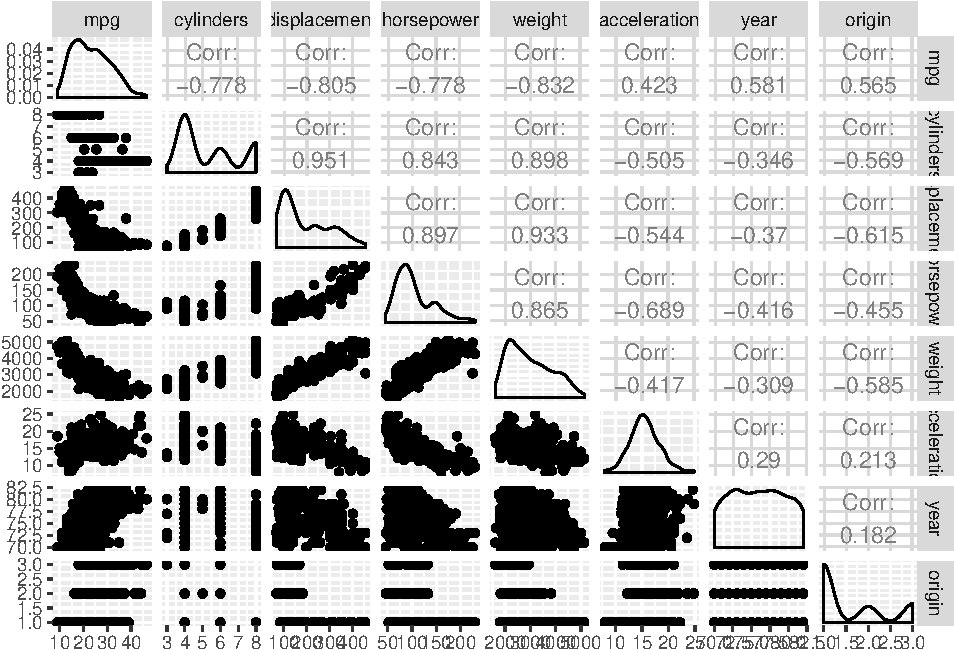
\includegraphics{3LinReg-sol_files/figure-latex/unnamed-chunk-3-1.pdf}

\begin{Shaded}
\begin{Highlighting}[]
\CommentTok{# qq-plot of residuals}
\KeywordTok{ggplot}\NormalTok{(modelB, }\KeywordTok{aes}\NormalTok{(}\DataTypeTok{sample =}\NormalTok{ .stdresid)) }\OperatorTok{+}
\StringTok{  }\KeywordTok{stat_qq}\NormalTok{(}\DataTypeTok{pch =} \DecValTok{19}\NormalTok{) }\OperatorTok{+}\StringTok{ }
\StringTok{  }\KeywordTok{geom_abline}\NormalTok{(}\DataTypeTok{intercept =} \DecValTok{0}\NormalTok{, }\DataTypeTok{slope =} \DecValTok{1}\NormalTok{, }\DataTypeTok{linetype =} \StringTok{"dotted"}\NormalTok{) }\OperatorTok{+}
\StringTok{  }\KeywordTok{labs}\NormalTok{(}\DataTypeTok{x =} \StringTok{"Theoretical quantiles"}\NormalTok{, }\DataTypeTok{y =} \StringTok{"Standardized residuals"}\NormalTok{, }\DataTypeTok{title =} \StringTok{"Normal Q-Q"}\NormalTok{, }\DataTypeTok{subtitle =} \KeywordTok{deparse}\NormalTok{(modelB}\OperatorTok{$}\NormalTok{call))}\OperatorTok{+}\StringTok{  }\KeywordTok{theme_minimal}\NormalTok{()}
\end{Highlighting}
\end{Shaded}

\includegraphics{3LinReg-sol_files/figure-latex/unnamed-chunk-3-2.pdf}

\begin{Shaded}
\begin{Highlighting}[]
\CommentTok{# normality test}
\KeywordTok{library}\NormalTok{(nortest) }
\KeywordTok{ad.test}\NormalTok{(}\KeywordTok{rstudent}\NormalTok{(modelB))}
\end{Highlighting}
\end{Shaded}

\begin{verbatim}
## 
##  Anderson-Darling normality test
## 
## data:  rstudent(modelB)
## A = 13.2, p-value < 2.2e-16
\end{verbatim}

\subsection{c) Confidence interval and hypothesis
test}\label{c-confidence-interval-and-hypothesis-test}

We use \texttt{modelA} and focus on addressing the association between
BMI and the response.

\begin{itemize}
\tightlist
\item
  What is the estimate \(\hat{\beta}_{\text{BMI}}\) (numerically)?
\item
  Explain how to interpret the estimated coefficient
  \(\hat{\beta}_{\text{BMI}}\).
\item
  Construct a 99\% confidence interval for \(\beta_{\text{BMI}}\) (write
  out the formula and calculate the interval numerically). Explain what
  this interval tells you.
\item
  From this confidence interval, is it possible for you know anything
  about the value of the \(p\)-value for the test
  \(H_0: \beta_{\text{BMI}}=0\) vs. \(H_1:\beta_{\text{BMI}} \neq 0\)?
  Explain.
\end{itemize}

\subsubsection{Answers:}\label{answers-2}

\begin{itemize}
\tightlist
\item
   \(\hat\beta = (X^TX)^{-1}X^TY\). From the summary output we find that
  \(\hat{\beta}_{\text{BMI}} = 0.0003\). This is the average increase in
  \(-1/sqrt(SYSBP)\) for a unit increase in BMI. Hence, keeping all
  other covariates fixed - having a BMI of 24 instead of 23, the value
  of \(-1/sqrt(SYSBP)\) will on average increase with 0.0003.
\item
  For linear regression where the distribution of the estimated
  coefficients are assumed to follow a t-distribution, we have that the
  \((1-\alpha)100\)\%-confidence interval is given by

  \begin{align*}
    \hat \beta \pm t_{\alpha/2, df} SD(\hat\beta)
  \end{align*}

  For \(\hat\beta_{BMI}\) the 99\% confidence interval is hence given by

  \begin{align*}
    [\hat \beta_{BMI} - t_{0.005, n-p-1} SD(\hat\beta_{BMI}), \hat \beta_{BMI} + t_{0.005, n-p-1} SD(\hat\beta_{BMI})] \\
  \end{align*}

  This means that before we have collected the data this interval has a
  99\% chance of covering the true value of \(\beta_{BMI}\). After the
  interval is made - now this is {[}0.00023, 0.00038{]} the the true
  value is either within the interval or not. But, colleting new data
  and making 99\% CIs, then 99\% of these will on average cover the true
  \(\beta_{BMI}\).
\item
  Since the interval does not cover 0, we know that the p-value is less
  than 0.01.
\end{itemize}

\begin{Shaded}
\begin{Highlighting}[]
\NormalTok{n =}\StringTok{ }\KeywordTok{dim}\NormalTok{(data)[}\DecValTok{1}\NormalTok{]}
\NormalTok{p =}\StringTok{ }\KeywordTok{dim}\NormalTok{(data)[}\DecValTok{2}\NormalTok{]}\OperatorTok{-}\DecValTok{1}
\NormalTok{betahat=modelA}\OperatorTok{$}\NormalTok{coefficients[}\DecValTok{5}\NormalTok{]}
\NormalTok{sdbetahat=}\KeywordTok{summary}\NormalTok{(modelA)}\OperatorTok{$}\NormalTok{coeff[}\DecValTok{5}\NormalTok{,}\DecValTok{2}\NormalTok{]}
\NormalTok{UCI =}\StringTok{ }\NormalTok{betahat }\OperatorTok{+}\StringTok{ }\KeywordTok{qt}\NormalTok{(}\FloatTok{0.005}\NormalTok{, }\DataTypeTok{df =}\NormalTok{ n}\OperatorTok{-}\NormalTok{p}\OperatorTok{-}\DecValTok{1}\NormalTok{, }\DataTypeTok{lower.tail =}\NormalTok{ F)}\OperatorTok{*}\NormalTok{sdbetahat}
\NormalTok{LCI =}\StringTok{ }\NormalTok{betahat }\OperatorTok{-}\StringTok{ }\KeywordTok{qt}\NormalTok{(}\FloatTok{0.005}\NormalTok{, }\DataTypeTok{df =}\NormalTok{ n}\OperatorTok{-}\NormalTok{p}\OperatorTok{-}\DecValTok{1}\NormalTok{, }\DataTypeTok{lower.tail =}\NormalTok{ F)}\OperatorTok{*}\NormalTok{sdbetahat}
\KeywordTok{c}\NormalTok{(LCI, UCI)}
\end{Highlighting}
\end{Shaded}

\begin{verbatim}
##          BMI          BMI 
## 0.0002325459 0.0003848866
\end{verbatim}

\subsection{d) Prediction}\label{d-prediction}

Consider a 56 year old man who is smoking. He is 1.75 meters tall and
his weight is 89 kilograms. His serum total cholesterol is 200 mg/dl and
he is not using anti-hypertensive medication.

\begin{Shaded}
\begin{Highlighting}[]
\KeywordTok{names}\NormalTok{(data)}
\end{Highlighting}
\end{Shaded}

\begin{verbatim}
## [1] "SYSBP"    "SEX"      "AGE"      "CURSMOKE" "BMI"      "TOTCHOL" 
## [7] "BPMEDS"
\end{verbatim}

\begin{Shaded}
\begin{Highlighting}[]
\NormalTok{new=}\KeywordTok{data.frame}\NormalTok{(}\DataTypeTok{SEX=}\DecValTok{1}\NormalTok{,}\DataTypeTok{AGE=}\DecValTok{56}\NormalTok{,}\DataTypeTok{CURSMOKE=}\DecValTok{1}\NormalTok{,}\DataTypeTok{BMI=}\DecValTok{89}\OperatorTok{/}\FloatTok{1.75}\OperatorTok{^}\DecValTok{2}\NormalTok{,}\DataTypeTok{TOTCHOL=}\DecValTok{200}\NormalTok{,}\DataTypeTok{BPMEDS=}\DecValTok{0}\NormalTok{)}
\end{Highlighting}
\end{Shaded}

\begin{itemize}
\tightlist
\item
  What is your best guess for his \texttt{-1/sqrt(SYSBP)}? To get a best
  guess for his \texttt{SYSBP} you may take the inverse function of
  \texttt{-1/sqrt} (this would be a first order Taylor expansion).
\item
  Construct a 90\% prediction interval for his systolic blood pressure
  \texttt{SYSBP}. Comment. Hint: first contruct values on the scale of
  the response \texttt{-1/sqrt(SYSBP)} and then transform the upper and
  lower limits of the prediction interval.
\item
  Do you find this prediction interval useful? Comment.
\end{itemize}

\subsubsection{Answers:}\label{answers-3}

{ Find best guess by prediction, and 90\% prediction interval.}

\begin{Shaded}
\begin{Highlighting}[]
\NormalTok{pred =}\StringTok{ }\KeywordTok{predict}\NormalTok{(modelA, }\DataTypeTok{newdata =}\NormalTok{ new)}
\NormalTok{pred}
\end{Highlighting}
\end{Shaded}

\begin{verbatim}
##           1 
## -0.08667246
\end{verbatim}

\begin{Shaded}
\begin{Highlighting}[]
\NormalTok{f.inv =}\StringTok{ }\ControlFlowTok{function}\NormalTok{(x) }\DecValTok{1}\OperatorTok{/}\NormalTok{x}\OperatorTok{^}\DecValTok{2}
\NormalTok{sys =}\StringTok{ }\KeywordTok{f.inv}\NormalTok{(pred)}
\CommentTok{#pred. interval}
\NormalTok{f.ci =}\StringTok{ }\KeywordTok{predict}\NormalTok{(modelA, }\DataTypeTok{newdata =}\NormalTok{ new, }\DataTypeTok{level =} \FloatTok{0.9}\NormalTok{, }\DataTypeTok{interval =} \StringTok{"prediction"}\NormalTok{)}
\NormalTok{f.ci}
\end{Highlighting}
\end{Shaded}

\begin{verbatim}
##           fit         lwr         upr
## 1 -0.08667246 -0.09625664 -0.07708829
\end{verbatim}

\begin{Shaded}
\begin{Highlighting}[]
\NormalTok{sys.ci =}\StringTok{ }\KeywordTok{f.inv}\NormalTok{(f.ci)}
\NormalTok{sys.ci}
\end{Highlighting}
\end{Shaded}

\begin{verbatim}
##        fit      lwr      upr
## 1 133.1183 107.9291 168.2764
\end{verbatim}

This prediction interval is very large and doesn't really tell us much.
A person with our characteristics on average has a 90\% chance of having
a systolic blood pressure between 108 and 168, and looking at the table
given in
\url{http://www.heart.org/HEARTORG/Conditions/HighBloodPressure/KnowYourNumbers/Understanding-Blood-Pressure-Readings_UCM_301764_Article.jsp\#.WnLqWOYo_AI},
we sse that this interval covers almost all the levels from normal to
high blood pressure. It seems our model is better for inference than
prediction.

\section{Problem 2}\label{problem-2}

\subsection{a)}\label{a}

\begin{align}
E(\hat{\boldsymbol\beta})&=E((X^T X)^{-1}X^T Y)=(X^TX)^{-1}X^T E(Y) =(X^TX)^{-1}X^T E(X \boldsymbol\beta +\epsilon) \\
&=(X^TX)^{-1}X^T (X \boldsymbol\beta +0)=(X^TX)^{-1}(X^T X) \boldsymbol\beta = I \boldsymbol\beta = \boldsymbol\beta
\end{align}

\begin{align}
Cov(\hat{\boldsymbol\beta})&=Cov((X^T X)^{-1}X^T Y)=(X^TX)^{-1}X^T Cov(Y)((X^TX)^{-1}X^T)^T \\
&=(X^TX)^{-1}X^T \sigma^2  I ((X^TX)^{-1}X^T)^T\\
&=\sigma^2 (X^TX)^{-1} \\
\end{align}

We need to assume that \(Y\) is multivariate normal. As
\(\hat{\boldsymbol\beta}\) is a linear transformation of a multivariate
normal vector \(Y\), \(\hat{\boldsymbol\beta}\) is also multivariate
normal.

The components of a multivariate normal vector, is univariate normal.
This means that \(\hat{\beta}_j\) is normally distributed with expected
value given by the \(\beta_j\) and the variance given by the \(j\)'th
diagonal element of \(\sigma^2 (X^T X)^{-1}\).

\subsection{b)}\label{b}

Fix covariates X. *Collect \(Y\), create CI using \(\hat{\beta}\) and
\(\hat{\sigma}\)*, repeat from * to * many times. 95 \% of the times the
CI contains the true \(\beta\). Collect \(Y\) means simulate it with the
true \(\beta\) as parameter(s). See also \texttt{R} code below.

\subsection{c)}\label{c}

Same idea. Fix covariates X and \(x_0\). *Collect \(Y\), create PI using
\(\hat{\beta}\) and \(\hat{\sigma}\), simulate \(Y_0\)*, repeat from *
to * many times. 95 \% of the times the PI contains \(Y_0\). Collect
\(Y\) and \(Y_0\) means simulate it with the true \(\beta\) as
parameter(s). \(Y_0\) should not be used to estimate \(\beta\) or
\(\sigma\). See also \texttt{R} code below.

\subsection{d)}\label{d}

95 \% CI for \(\mathbf{x}_0^T\mathbf{\beta}\): Same idea as for
\(\beta_j\). Use that
\(\mathbf{x}_0^T\hat{\mathbf{\beta}} \sim N(\mathbf{x}_0^T\mathbf{\beta}, \mathbf{x}_0^T\)Var\((\hat{\mathbf{\beta}})\mathbf{x}_0)\)
and do as for \(\beta_j\). Note that \(\mathbf{x}_0\) is a vector. The
connection between CI for \(\mathbf{\beta}\),
\(\mathbf{x}_0^T\mathbf{\beta}\) and PI for \(Y\) at \(\mathbf{x}_0\):
The first is CI for a parameter, the second is CI for the expected
regression line in the point \(x_0\) (when you only have one covariate,
this may be more intuitive), and the last is the PI for the response
\(Y_0\). The difference between the two latter is that \(Y\) are the
observations, and \(\mathbf{x}_0^T\mathbf{\beta}\) is the expected value
of the observations and hence a function of the model parameters (NOT an
observation).

\subsection{e)}\label{e}

We have a model on the form \(Y=X \beta + \epsilon\) where \(\epsilon\)
is the error. The error of the model is unknown and unobserved, but we
can estimate it by what we call the residuals. The residuals are given
by the difference between the true response and the predicted value
\[\hat{\epsilon}=Y-\hat{Y}=(I-X(X^TX)^{-1}X^T)Y.\]

Properties of raw residuals: Normally distributed with mean 0 and
covariance \(Cov(\hat{\epsilon})=\sigma^2 (I-X(X^TX)^{-1}X^T).\) This
means that the residuals may have different variance (depending on
\(X\)) and may also be correlated.

In a model check, we want to check that our errors are independent,
homoscedastic (same variance for each observation) and not dependent on
the covariates. As we don't know the true error, we use the residuals as
predictors, but as mentioned, the residuals may have different variances
and may be correlated. This is why we don't want to use the raw
residuals for model check.

To amend our problem we need to try to fix the residuals so that they at
least have equal variances. We do that by working with standardized or
studentized residuals.

\subsection{f)}\label{f}

RSS(small) \(\geq\) RSS(large) since RSS will be smaller with more
covariates explaining the variation (and for a covariate that is
completly unrelated to the data it might not be a large change, but the
RSS will not increase). \(R^2\) is directly related to RSS: \(R^2 = 1\)
- RSS/TSS, and TSS does not change when the model changes.

\section{Problem 3: Munich Rent
index}\label{problem-3-munich-rent-index}

\subsection{a)}\label{a-1}

\begin{Shaded}
\begin{Highlighting}[]
\KeywordTok{library}\NormalTok{(ggplot2)}
\KeywordTok{library}\NormalTok{(gamlss.data)}
\KeywordTok{library}\NormalTok{(dplyr)}
\KeywordTok{data}\NormalTok{(}\StringTok{"rent99"}\NormalTok{)}

\NormalTok{rent99}\OperatorTok{$}\NormalTok{location=}\KeywordTok{as.factor}\NormalTok{(rent99}\OperatorTok{$}\NormalTok{location)}
\NormalTok{formula1 <-}\StringTok{ }\NormalTok{rent }\OperatorTok{~}\StringTok{ }\NormalTok{area }\OperatorTok{+}\NormalTok{location }\OperatorTok{+}\StringTok{ }\NormalTok{bath }\OperatorTok{+}\StringTok{ }\NormalTok{kitchen }\OperatorTok{+}\StringTok{ }\NormalTok{cheating}
\NormalTok{formula2 <-}\StringTok{ }\NormalTok{rentsqm }\OperatorTok{~}\StringTok{ }\NormalTok{area }\OperatorTok{+}\StringTok{ }\NormalTok{location }\OperatorTok{+}\StringTok{ }\NormalTok{bath }\OperatorTok{+}\StringTok{ }\NormalTok{kitchen }\OperatorTok{+}\StringTok{ }\NormalTok{cheating}

\NormalTok{rent1 <-}\StringTok{ }\KeywordTok{lm}\NormalTok{(formula1,}\DataTypeTok{data=}\NormalTok{rent99)}
\NormalTok{rent2<-}\KeywordTok{lm}\NormalTok{(formula2,}\DataTypeTok{data=}\NormalTok{rent99)}
\end{Highlighting}
\end{Shaded}

Look at the summary

\begin{Shaded}
\begin{Highlighting}[]
\KeywordTok{summary}\NormalTok{(rent1)}
\end{Highlighting}
\end{Shaded}

\begin{verbatim}
## 
## Call:
## lm(formula = formula1, data = rent99)
## 
## Residuals:
##     Min      1Q  Median      3Q     Max 
## -633.41  -89.17   -6.26   82.96 1000.76 
## 
## Coefficients:
##             Estimate Std. Error t value Pr(>|t|)    
## (Intercept) -21.9733    11.6549  -1.885   0.0595 .  
## area          4.5788     0.1143  40.055  < 2e-16 ***
## location2    39.2602     5.4471   7.208 7.14e-13 ***
## location3   126.0575    16.8747   7.470 1.04e-13 ***
## bath1        74.0538    11.2087   6.607 4.61e-11 ***
## kitchen1    120.4349    13.0192   9.251  < 2e-16 ***
## cheating1   161.4138     8.6632  18.632  < 2e-16 ***
## ---
## Signif. codes:  0 '***' 0.001 '**' 0.01 '*' 0.05 '.' 0.1 ' ' 1
## 
## Residual standard error: 145.2 on 3075 degrees of freedom
## Multiple R-squared:  0.4504, Adjusted R-squared:  0.4494 
## F-statistic:   420 on 6 and 3075 DF,  p-value: < 2.2e-16
\end{verbatim}

\begin{Shaded}
\begin{Highlighting}[]
\KeywordTok{summary}\NormalTok{(rent2)}
\end{Highlighting}
\end{Shaded}

\begin{verbatim}
## 
## Call:
## lm(formula = formula2, data = rent99)
## 
## Residuals:
##     Min      1Q  Median      3Q     Max 
## -7.4959 -1.4084 -0.0733  1.3847  9.4400 
## 
## Coefficients:
##              Estimate Std. Error t value Pr(>|t|)    
## (Intercept)  7.108319   0.168567  42.169  < 2e-16 ***
## area        -0.038154   0.001653 -23.077  < 2e-16 ***
## location2    0.628698   0.078782   7.980 2.04e-15 ***
## location3    1.686099   0.244061   6.909 5.93e-12 ***
## bath1        0.989898   0.162113   6.106 1.15e-09 ***
## kitchen1     1.412113   0.188299   7.499 8.34e-14 ***
## cheating1    2.414101   0.125297  19.267  < 2e-16 ***
## ---
## Signif. codes:  0 '***' 0.001 '**' 0.01 '*' 0.05 '.' 0.1 ' ' 1
## 
## Residual standard error: 2.1 on 3075 degrees of freedom
## Multiple R-squared:  0.2584, Adjusted R-squared:  0.2569 
## F-statistic: 178.6 on 6 and 3075 DF,  p-value: < 2.2e-16
\end{verbatim}

Consider residual plots. We plot standardized residuals against fitted
values.

\begin{Shaded}
\begin{Highlighting}[]
\NormalTok{yhat1=}\KeywordTok{predict}\NormalTok{(rent1)}
\NormalTok{yhat2=}\KeywordTok{predict}\NormalTok{(rent2)}

\NormalTok{estand1=}\KeywordTok{rstandard}\NormalTok{(rent1);}
\NormalTok{estand2=}\KeywordTok{rstandard}\NormalTok{(rent2)}
 
\KeywordTok{ggplot}\NormalTok{(}\KeywordTok{data.frame}\NormalTok{(yhat1,estand1),}\KeywordTok{aes}\NormalTok{(yhat1,estand1))}\OperatorTok{+}\KeywordTok{geom_point}\NormalTok{(}\DataTypeTok{pch=}\DecValTok{19}\NormalTok{)}\OperatorTok{+}\KeywordTok{geom_abline}\NormalTok{(}\DataTypeTok{intercept=}\DecValTok{0}\NormalTok{,}\DataTypeTok{slope=}\DecValTok{0}\NormalTok{,}\DataTypeTok{col=}\StringTok{"red"}\NormalTok{)}\OperatorTok{+}\StringTok{  }\KeywordTok{theme_minimal}\NormalTok{()}
\end{Highlighting}
\end{Shaded}

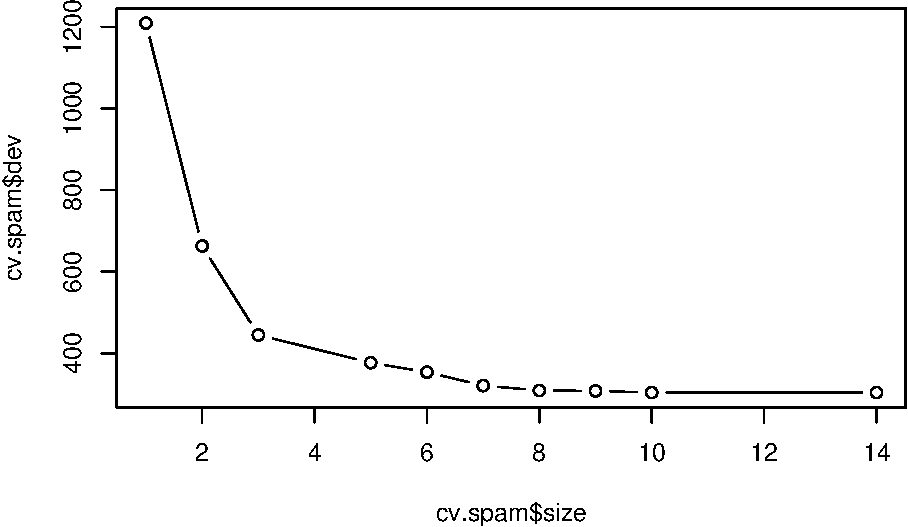
\includegraphics{3LinReg-sol_files/figure-latex/unnamed-chunk-9-1.pdf}

\begin{Shaded}
\begin{Highlighting}[]
\KeywordTok{ggplot}\NormalTok{(}\KeywordTok{data.frame}\NormalTok{(yhat2,estand2),}\KeywordTok{aes}\NormalTok{(yhat2,estand2))}\OperatorTok{+}\KeywordTok{geom_point}\NormalTok{(}\DataTypeTok{pch=}\DecValTok{19}\NormalTok{)}\OperatorTok{+}\KeywordTok{geom_abline}\NormalTok{(}\DataTypeTok{intercept=}\DecValTok{0}\NormalTok{,}\DataTypeTok{slope=}\DecValTok{0}\NormalTok{,}\DataTypeTok{col=}\StringTok{"red"}\NormalTok{)}\OperatorTok{+}\StringTok{  }\KeywordTok{theme_minimal}\NormalTok{()}
\end{Highlighting}
\end{Shaded}

\includegraphics{3LinReg-sol_files/figure-latex/unnamed-chunk-9-2.pdf}

We plot the true observations against the fitted values

\begin{Shaded}
\begin{Highlighting}[]
\KeywordTok{ggplot}\NormalTok{(}\KeywordTok{data.frame}\NormalTok{(yhat1,rent99),}\KeywordTok{aes}\NormalTok{(rent99}\OperatorTok{$}\NormalTok{rent,yhat1))}\OperatorTok{+}\KeywordTok{geom_point}\NormalTok{(}\DataTypeTok{pch=}\DecValTok{19}\NormalTok{)}\OperatorTok{+}\KeywordTok{geom_abline}\NormalTok{(}\DataTypeTok{intercept=}\DecValTok{0}\NormalTok{,}\DataTypeTok{slope=}\DecValTok{1}\NormalTok{,}\DataTypeTok{col=}\StringTok{"red"}\NormalTok{)}\OperatorTok{+}\StringTok{  }\KeywordTok{theme_minimal}\NormalTok{()}
\end{Highlighting}
\end{Shaded}

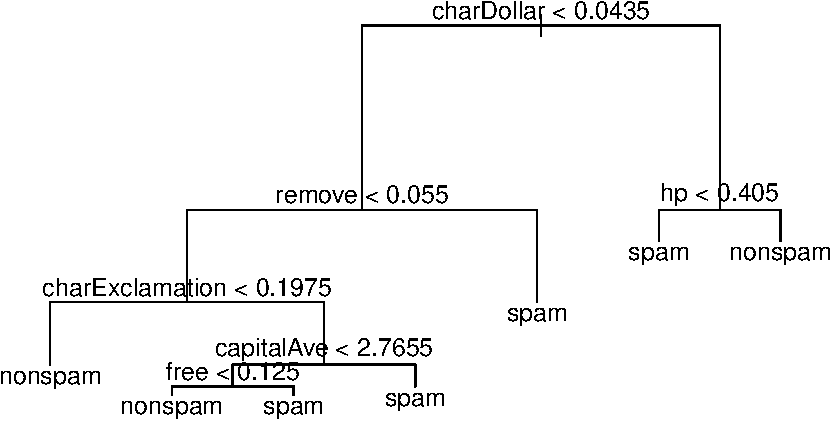
\includegraphics{3LinReg-sol_files/figure-latex/unnamed-chunk-10-1.pdf}

\begin{Shaded}
\begin{Highlighting}[]
\KeywordTok{ggplot}\NormalTok{(}\KeywordTok{data.frame}\NormalTok{(yhat2,rent99),}\KeywordTok{aes}\NormalTok{(rent99}\OperatorTok{$}\NormalTok{rentsqm,yhat2))}\OperatorTok{+}\KeywordTok{geom_point}\NormalTok{(}\DataTypeTok{pch=}\DecValTok{19}\NormalTok{)}\OperatorTok{+}\KeywordTok{geom_abline}\NormalTok{(}\DataTypeTok{intercept=}\DecValTok{0}\NormalTok{,}\DataTypeTok{slope=}\DecValTok{1}\NormalTok{,}\DataTypeTok{col=}\StringTok{"red"}\NormalTok{)}\OperatorTok{+}\StringTok{  }\KeywordTok{theme_minimal}\NormalTok{()}
\end{Highlighting}
\end{Shaded}

\includegraphics{3LinReg-sol_files/figure-latex/unnamed-chunk-10-2.pdf}

Normal Q-Q

\begin{Shaded}
\begin{Highlighting}[]
\KeywordTok{ggplot}\NormalTok{(rent1, }\KeywordTok{aes}\NormalTok{(}\DataTypeTok{sample =}\NormalTok{ .stdresid)) }\OperatorTok{+}
\StringTok{  }\KeywordTok{stat_qq}\NormalTok{(}\DataTypeTok{pch =} \DecValTok{19}\NormalTok{) }\OperatorTok{+}
\StringTok{  }\KeywordTok{geom_abline}\NormalTok{(}\DataTypeTok{intercept =} \DecValTok{0}\NormalTok{, }\DataTypeTok{slope =} \DecValTok{1}\NormalTok{, }\DataTypeTok{linetype =} \StringTok{"dotted"}\NormalTok{) }\OperatorTok{+}
\StringTok{  }\KeywordTok{labs}\NormalTok{(}\DataTypeTok{x =} \StringTok{"Theoretical quantiles"}\NormalTok{, }\DataTypeTok{y =} \StringTok{"Standardized residuals"}\NormalTok{, }\DataTypeTok{title =} \StringTok{"Normal Q-Q"}\NormalTok{, }\DataTypeTok{subtitle =} \KeywordTok{deparse}\NormalTok{(rent1}\OperatorTok{$}\NormalTok{call))}\OperatorTok{+}\StringTok{  }\KeywordTok{theme_minimal}\NormalTok{()}
\end{Highlighting}
\end{Shaded}

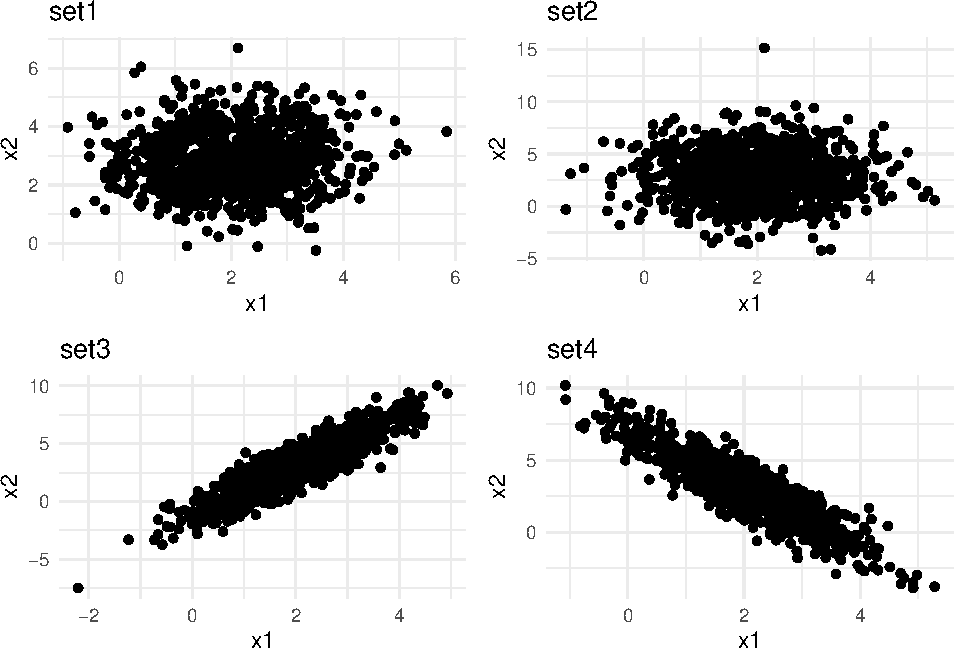
\includegraphics{3LinReg-sol_files/figure-latex/unnamed-chunk-11-1.pdf}

\begin{Shaded}
\begin{Highlighting}[]
\KeywordTok{ggplot}\NormalTok{(rent2, }\KeywordTok{aes}\NormalTok{(}\DataTypeTok{sample =}\NormalTok{ .stdresid)) }\OperatorTok{+}
\StringTok{  }\KeywordTok{stat_qq}\NormalTok{(}\DataTypeTok{pch =} \DecValTok{19}\NormalTok{) }\OperatorTok{+}
\StringTok{  }\KeywordTok{geom_abline}\NormalTok{(}\DataTypeTok{intercept =} \DecValTok{0}\NormalTok{, }\DataTypeTok{slope =} \DecValTok{1}\NormalTok{, }\DataTypeTok{linetype =} \StringTok{"dotted"}\NormalTok{) }\OperatorTok{+}
\StringTok{  }\KeywordTok{labs}\NormalTok{(}\DataTypeTok{x =} \StringTok{"Theoretical quantiles"}\NormalTok{, }\DataTypeTok{y =} \StringTok{"Standardized residuals"}\NormalTok{, }\DataTypeTok{title =} \StringTok{"Normal Q-Q"}\NormalTok{, }\DataTypeTok{subtitle =} \KeywordTok{deparse}\NormalTok{(rent2}\OperatorTok{$}\NormalTok{call))}\OperatorTok{+}\StringTok{  }\KeywordTok{theme_minimal}\NormalTok{()}
\end{Highlighting}
\end{Shaded}

\includegraphics{3LinReg-sol_files/figure-latex/unnamed-chunk-11-2.pdf}

Can't really see that one response is better than the other, so we
proceed with \(rent\).

\subsection{b\&c)}\label{bc}

We consider the summary

\begin{Shaded}
\begin{Highlighting}[]
\KeywordTok{summary}\NormalTok{(rent1)}
\end{Highlighting}
\end{Shaded}

\begin{verbatim}
## 
## Call:
## lm(formula = formula1, data = rent99)
## 
## Residuals:
##     Min      1Q  Median      3Q     Max 
## -633.41  -89.17   -6.26   82.96 1000.76 
## 
## Coefficients:
##             Estimate Std. Error t value Pr(>|t|)    
## (Intercept) -21.9733    11.6549  -1.885   0.0595 .  
## area          4.5788     0.1143  40.055  < 2e-16 ***
## location2    39.2602     5.4471   7.208 7.14e-13 ***
## location3   126.0575    16.8747   7.470 1.04e-13 ***
## bath1        74.0538    11.2087   6.607 4.61e-11 ***
## kitchen1    120.4349    13.0192   9.251  < 2e-16 ***
## cheating1   161.4138     8.6632  18.632  < 2e-16 ***
## ---
## Signif. codes:  0 '***' 0.001 '**' 0.01 '*' 0.05 '.' 0.1 ' ' 1
## 
## Residual standard error: 145.2 on 3075 degrees of freedom
## Multiple R-squared:  0.4504, Adjusted R-squared:  0.4494 
## F-statistic:   420 on 6 and 3075 DF,  p-value: < 2.2e-16
\end{verbatim}

The column \emph{estimate} gives us the \(\hat{\beta}\)'s. For example
if the living area of the house increases qith 1 square meter, the
predicted response, net rent per month, increases with \(4.5788\) euro.
The column std.error gives the standard deviation of the
\(\hat{\beta}\)'s. The remaining columns report the t value (\emph{t
value}) with corresponding p-value
(\emph{Pr(\textgreater{}\textbar{}t\textbar{})}). The \(RSE\), \(R^2\),
\(R_{adj}^2\) and \(F\)-statistic are also reported as \emph{Residual
standard error}, \emph{Multiple R-squared}, \emph{Adjusted R-Squared}
and \emph{F-statistic} respectively. See module page for definition of
these terms.

Interpretation of the intercept: This is the intercept of a average
location (location=1). (If location=2, the intercept is
-21.9733+39.2602, and if location=3 the intercept is -21.9733+126.0575.)

\subsection{d)}\label{d-1}

\begin{Shaded}
\begin{Highlighting}[]
\NormalTok{orgfit=}\KeywordTok{lm}\NormalTok{(rent}\OperatorTok{~}\NormalTok{area}\OperatorTok{+}\NormalTok{location}\OperatorTok{+}\NormalTok{bath}\OperatorTok{+}\NormalTok{kitchen}\OperatorTok{+}\NormalTok{cheating,}\DataTypeTok{data=}\NormalTok{rent99)}
\KeywordTok{summary}\NormalTok{(orgfit)}
\KeywordTok{set.seed}\NormalTok{(}\DecValTok{1}\NormalTok{) }\CommentTok{#to be able to reproduce results}
\NormalTok{n=}\KeywordTok{dim}\NormalTok{(rent99)[}\DecValTok{1}\NormalTok{]}
\NormalTok{IQ=}\KeywordTok{rnorm}\NormalTok{(n,}\DecValTok{100}\NormalTok{,}\DecValTok{16}\NormalTok{)}
\NormalTok{fitIQ=}\KeywordTok{lm}\NormalTok{(rent}\OperatorTok{~}\NormalTok{area}\OperatorTok{+}\KeywordTok{as.factor}\NormalTok{(location)}\OperatorTok{+}\NormalTok{bath}\OperatorTok{+}\NormalTok{kitchen}\OperatorTok{+}\NormalTok{cheating}\OperatorTok{+}\NormalTok{IQ,}\DataTypeTok{data=}\NormalTok{rent99)}
\KeywordTok{summary}\NormalTok{(fitIQ)}

\KeywordTok{summary}\NormalTok{(orgfit)}\OperatorTok{$}\NormalTok{sigma}
\KeywordTok{summary}\NormalTok{(fitIQ)}\OperatorTok{$}\NormalTok{sigma}

\KeywordTok{summary}\NormalTok{(orgfit)}\OperatorTok{$}\NormalTok{r.squared}
\KeywordTok{summary}\NormalTok{(fitIQ)}\OperatorTok{$}\NormalTok{r.squared}
\KeywordTok{summary}\NormalTok{(orgfit)}\OperatorTok{$}\NormalTok{adj.r.squared}
\KeywordTok{summary}\NormalTok{(fitIQ)}\OperatorTok{$}\NormalTok{adj.r.squared}
\end{Highlighting}
\end{Shaded}

\begin{verbatim}
## 
## Call:
## lm(formula = rent ~ area + location + bath + kitchen + cheating, 
##     data = rent99)
## 
## Residuals:
##     Min      1Q  Median      3Q     Max 
## -633.41  -89.17   -6.26   82.96 1000.76 
## 
## Coefficients:
##             Estimate Std. Error t value Pr(>|t|)    
## (Intercept) -21.9733    11.6549  -1.885   0.0595 .  
## area          4.5788     0.1143  40.055  < 2e-16 ***
## location2    39.2602     5.4471   7.208 7.14e-13 ***
## location3   126.0575    16.8747   7.470 1.04e-13 ***
## bath1        74.0538    11.2087   6.607 4.61e-11 ***
## kitchen1    120.4349    13.0192   9.251  < 2e-16 ***
## cheating1   161.4138     8.6632  18.632  < 2e-16 ***
## ---
## Signif. codes:  0 '***' 0.001 '**' 0.01 '*' 0.05 '.' 0.1 ' ' 1
## 
## Residual standard error: 145.2 on 3075 degrees of freedom
## Multiple R-squared:  0.4504, Adjusted R-squared:  0.4494 
## F-statistic:   420 on 6 and 3075 DF,  p-value: < 2.2e-16
## 
## 
## Call:
## lm(formula = rent ~ area + as.factor(location) + bath + kitchen + 
##     cheating + IQ, data = rent99)
## 
## Residuals:
##     Min      1Q  Median      3Q     Max 
## -630.95  -89.50   -6.12   82.62  995.76 
## 
## Coefficients:
##                      Estimate Std. Error t value Pr(>|t|)    
## (Intercept)          -41.3879    19.5957  -2.112   0.0348 *  
## area                   4.5785     0.1143  40.056  < 2e-16 ***
## as.factor(location)2  39.2830     5.4467   7.212 6.90e-13 ***
## as.factor(location)3 126.3356    16.8748   7.487 9.18e-14 ***
## bath1                 74.1979    11.2084   6.620 4.23e-11 ***
## kitchen1             120.0756    13.0214   9.221  < 2e-16 ***
## cheating1            161.4450     8.6625  18.637  < 2e-16 ***
## IQ                     0.1940     0.1574   1.232   0.2179    
## ---
## Signif. codes:  0 '***' 0.001 '**' 0.01 '*' 0.05 '.' 0.1 ' ' 1
## 
## Residual standard error: 145.2 on 3074 degrees of freedom
## Multiple R-squared:  0.4507, Adjusted R-squared:  0.4494 
## F-statistic: 360.3 on 7 and 3074 DF,  p-value: < 2.2e-16
## 
## [1] 145.1879
## [1] 145.1757
## [1] 0.4504273
## [1] 0.4506987
## [1] 0.449355
## [1] 0.4494479
\end{verbatim}

\(R^2\) will always increase (or stay the same) if we add a parameter to
the model. Thus, we cannot use this alone for model selection. However,
the adjusted \(R_{adj}^2\) is ``punished'' based on the number of
parameters in the model and will not necessarily increase if we add a
covariate to the model.

Sigma (or RSE) is given by \(\hat{\sigma}=\sqrt{\frac{1}{n-p-1}RSS}\).
Multiple R-squared is given by
\(R^2=1-\frac{RSS}{TSS}=1-\frac{\hat{\sigma}^2 (n-p-1)}{TSS}\).

\subsection{e)}\label{e-1}

\begin{Shaded}
\begin{Highlighting}[]
\NormalTok{formula <-}\StringTok{ }\NormalTok{rent }\OperatorTok{~}\StringTok{ }\NormalTok{area }\OperatorTok{+}\StringTok{ }\NormalTok{location }\OperatorTok{+}\StringTok{ }\NormalTok{bath }\OperatorTok{+}\StringTok{ }\NormalTok{kitchen }\OperatorTok{+}\StringTok{ }\NormalTok{cheating}
\NormalTok{rent1 <-}\StringTok{ }\KeywordTok{lm}\NormalTok{(formula, }\DataTypeTok{data =}\NormalTok{ rent99)}\CommentTok{#, contrasts = list(location = "contr.sum"))}

\NormalTok{rent99 <-}\StringTok{ }\NormalTok{rent99 }\OperatorTok\StringTok{ }\KeywordTok{mutate}\NormalTok{(}\DataTypeTok{yearc.cat =} \KeywordTok{cut}\NormalTok{(yearc, }\DataTypeTok{breaks =} \KeywordTok{c}\NormalTok{(}\OperatorTok{-}\OtherTok{Inf}\NormalTok{, }\KeywordTok{seq}\NormalTok{(}\DecValTok{1920}\NormalTok{,}\DecValTok{2000}\NormalTok{,}\DecValTok{10}\NormalTok{)), }\DataTypeTok{labels =} \DecValTok{10}\OperatorTok{*}\DecValTok{1}\OperatorTok{:}\DecValTok{9}\NormalTok{))}

\NormalTok{formula <-}\StringTok{ }\NormalTok{rent }\OperatorTok{~}\StringTok{ }\NormalTok{area }\OperatorTok{+}\StringTok{ }\NormalTok{location }\OperatorTok{+}\StringTok{ }\NormalTok{bath }\OperatorTok{+}\StringTok{ }\NormalTok{kitchen }\OperatorTok{+}\StringTok{ }\NormalTok{cheating }\OperatorTok{+}\StringTok{ }\NormalTok{yearc.cat}
\NormalTok{rent2 <-}\StringTok{ }\KeywordTok{lm}\NormalTok{(formula, }\DataTypeTok{data =}\NormalTok{ rent99)}\CommentTok{#, contrasts = list(location = "contr.sum"))}

\NormalTok{rent99 <-}\StringTok{ }\NormalTok{rent99 }\OperatorTok\StringTok{ }\KeywordTok{mutate}\NormalTok{(}\DataTypeTok{yearc.cat2 =} \KeywordTok{cut}\NormalTok{(yearc, }\DataTypeTok{breaks =} \KeywordTok{c}\NormalTok{(}\OperatorTok{-}\OtherTok{Inf}\NormalTok{, }\KeywordTok{seq}\NormalTok{(}\DecValTok{1920}\NormalTok{,}\DecValTok{2000}\NormalTok{,}\DecValTok{20}\NormalTok{)), }\DataTypeTok{labels =} \KeywordTok{c}\NormalTok{(}\DecValTok{20}\NormalTok{,}\DecValTok{40}\NormalTok{,}\DecValTok{60}\NormalTok{,}\DecValTok{80}\NormalTok{,}\DecValTok{00}\NormalTok{)))}

\NormalTok{formula <-}\StringTok{ }\NormalTok{rent }\OperatorTok{~}\StringTok{ }\NormalTok{area }\OperatorTok{+}\StringTok{ }\NormalTok{location }\OperatorTok{+}\StringTok{ }\NormalTok{bath }\OperatorTok{+}\StringTok{ }\NormalTok{kitchen }\OperatorTok{+}\StringTok{ }\NormalTok{cheating }\OperatorTok{+}\StringTok{ }\NormalTok{yearc.cat2}
\NormalTok{rent3 <-}\StringTok{ }\KeywordTok{lm}\NormalTok{(formula, }\DataTypeTok{data =}\NormalTok{ rent99)}\CommentTok{#,contrasts = list(location = "contr.sum"))}
\end{Highlighting}
\end{Shaded}

\subsection{f)}\label{f-1}

\begin{Shaded}
\begin{Highlighting}[]
\KeywordTok{library}\NormalTok{(MASS)}
\KeywordTok{library}\NormalTok{(leaps)}
\NormalTok{best <-}\StringTok{ }\KeywordTok{regsubsets}\NormalTok{(}\KeywordTok{model.matrix}\NormalTok{(rent3)[,}\OperatorTok{-}\DecValTok{1}\NormalTok{], }\DataTypeTok{y =}\NormalTok{ rent99}\OperatorTok{$}\NormalTok{rent,}\DataTypeTok{method=}\StringTok{"exhaustive"}\NormalTok{)}
\KeywordTok{summary}\NormalTok{(best)}
\end{Highlighting}
\end{Shaded}

\begin{verbatim}
## Subset selection object
## 10 Variables  (and intercept)
##              Forced in Forced out
## area             FALSE      FALSE
## location2        FALSE      FALSE
## location3        FALSE      FALSE
## bath1            FALSE      FALSE
## kitchen1         FALSE      FALSE
## cheating1        FALSE      FALSE
## yearc.cat240     FALSE      FALSE
## yearc.cat260     FALSE      FALSE
## yearc.cat280     FALSE      FALSE
## yearc.cat20      FALSE      FALSE
## 1 subsets of each size up to 8
## Selection Algorithm: exhaustive
##          area location2 location3 bath1 kitchen1 cheating1 yearc.cat240
## 1  ( 1 ) "*"  " "       " "       " "   " "      " "       " "         
## 2  ( 1 ) "*"  " "       " "       " "   " "      " "       " "         
## 3  ( 1 ) "*"  " "       " "       " "   " "      "*"       " "         
## 4  ( 1 ) "*"  " "       "*"       " "   " "      "*"       " "         
## 5  ( 1 ) "*"  "*"       "*"       " "   " "      "*"       " "         
## 6  ( 1 ) "*"  "*"       "*"       " "   " "      "*"       " "         
## 7  ( 1 ) "*"  "*"       "*"       " "   "*"      "*"       " "         
## 8  ( 1 ) "*"  "*"       "*"       "*"   "*"      "*"       " "         
##          yearc.cat260 yearc.cat280 yearc.cat20
## 1  ( 1 ) " "          " "          " "        
## 2  ( 1 ) " "          " "          "*"        
## 3  ( 1 ) " "          " "          "*"        
## 4  ( 1 ) " "          " "          "*"        
## 5  ( 1 ) " "          " "          "*"        
## 6  ( 1 ) " "          "*"          "*"        
## 7  ( 1 ) " "          "*"          "*"        
## 8  ( 1 ) " "          "*"          "*"
\end{verbatim}

A selection method is used (you will learn more later). The output shows
the best model of each size (1-8 covariates). The best model with one
covariate uses only area, the best model with two covariates uses area
and yearc.cat20 and so on.

\begin{Shaded}
\begin{Highlighting}[]
\KeywordTok{summary}\NormalTok{(best)}\OperatorTok{$}\NormalTok{cp}
\end{Highlighting}
\end{Shaded}

\begin{verbatim}
## [1] 1015.979023  540.680039  228.460243  184.179283  125.679898   75.667739
## [7]   32.571877    9.418625
\end{verbatim}

Model 8 gives the lowest Mallows Cp and is the preferred model.

\section{Problem 4: Simulations in R}\label{problem-4-simulations-in-r}

\subsection{a)}\label{a-2}

\begin{Shaded}
\begin{Highlighting}[]
\CommentTok{# CI for beta_j}

\NormalTok{true_beta <-}\StringTok{ }\KeywordTok{c}\NormalTok{(}\FloatTok{3.14}\NormalTok{, }\DecValTok{10}\NormalTok{, }\FloatTok{0.8}\NormalTok{) }\CommentTok{# choosing true betas}
\NormalTok{true_sd <-}\StringTok{ }\DecValTok{10} \CommentTok{# choosing true sd}
\KeywordTok{set.seed}\NormalTok{(}\DecValTok{345}\NormalTok{); X <-}\StringTok{ }\KeywordTok{matrix}\NormalTok{(}\KeywordTok{c}\NormalTok{(}\KeywordTok{rep}\NormalTok{(}\DecValTok{1}\NormalTok{, }\DecValTok{100}\NormalTok{), }\KeywordTok{runif}\NormalTok{(}\DecValTok{100}\NormalTok{, }\DecValTok{2}\NormalTok{, }\DecValTok{5}\NormalTok{), }\KeywordTok{sample}\NormalTok{(}\DecValTok{1}\OperatorTok{:}\DecValTok{100}\NormalTok{, }\DecValTok{100}\NormalTok{, }\DataTypeTok{replace =} \OtherTok{TRUE}\NormalTok{)), }
            \DataTypeTok{nrow =} \DecValTok{100}\NormalTok{, }\DataTypeTok{ncol =} \DecValTok{3}\NormalTok{) }\CommentTok{# fixing X. set.seed() is used to produce same X every time this code is used}

\CommentTok{# simulating and fitting models many times}
\NormalTok{ci_int <-}\StringTok{ }\NormalTok{ci_x1 <-}\StringTok{ }\NormalTok{ci_x2 <-}\StringTok{ }\DecValTok{0}\NormalTok{; nsim <-}\StringTok{ }\DecValTok{1000}
\ControlFlowTok{for}\NormalTok{ (i }\ControlFlowTok{in} \DecValTok{1}\OperatorTok{:}\NormalTok{nsim)\{}
\NormalTok{  y <-}\StringTok{ }\KeywordTok{rnorm}\NormalTok{(}\DataTypeTok{n =} \DecValTok{100}\NormalTok{, }\DataTypeTok{mean =}\NormalTok{ X}\OperatorTok\NormalTok{true_beta, }\DataTypeTok{sd =} \KeywordTok{rep}\NormalTok{(true_sd, }\DecValTok{100}\NormalTok{))}
\NormalTok{  mod <-}\StringTok{ }\KeywordTok{lm}\NormalTok{(y }\OperatorTok{~}\StringTok{ }\NormalTok{x1 }\OperatorTok{+}\StringTok{ }\NormalTok{x2, }\DataTypeTok{data =} \KeywordTok{data.frame}\NormalTok{(}\DataTypeTok{y =}\NormalTok{ y, }\DataTypeTok{x1 =}\NormalTok{ X[,}\DecValTok{2}\NormalTok{], }\DataTypeTok{x2 =}\NormalTok{ X[,}\DecValTok{3}\NormalTok{]))}
\NormalTok{  ci <-}\StringTok{ }\KeywordTok{confint}\NormalTok{(mod)}
\NormalTok{  ci_int[i] <-}\StringTok{ }\KeywordTok{ifelse}\NormalTok{(true_beta[}\DecValTok{1}\NormalTok{] }\OperatorTok{>=}\StringTok{ }\NormalTok{ci[}\DecValTok{1}\NormalTok{,}\DecValTok{1}\NormalTok{] }\OperatorTok{&&}\StringTok{ }\NormalTok{true_beta[}\DecValTok{1}\NormalTok{] }\OperatorTok{<=}\StringTok{ }\NormalTok{ci[}\DecValTok{1}\NormalTok{,}\DecValTok{2}\NormalTok{], }\DecValTok{1}\NormalTok{, }\DecValTok{0}\NormalTok{)}
\NormalTok{  ci_x1[i] <-}\StringTok{ }\KeywordTok{ifelse}\NormalTok{(true_beta[}\DecValTok{2}\NormalTok{] }\OperatorTok{>=}\StringTok{ }\NormalTok{ci[}\DecValTok{2}\NormalTok{,}\DecValTok{1}\NormalTok{] }\OperatorTok{&&}\StringTok{ }\NormalTok{true_beta[}\DecValTok{2}\NormalTok{] }\OperatorTok{<=}\StringTok{ }\NormalTok{ci[}\DecValTok{2}\NormalTok{,}\DecValTok{2}\NormalTok{], }\DecValTok{1}\NormalTok{, }\DecValTok{0}\NormalTok{)}
\NormalTok{  ci_x2[i] <-}\StringTok{ }\KeywordTok{ifelse}\NormalTok{(true_beta[}\DecValTok{3}\NormalTok{] }\OperatorTok{>=}\StringTok{ }\NormalTok{ci[}\DecValTok{3}\NormalTok{,}\DecValTok{1}\NormalTok{] }\OperatorTok{&&}\StringTok{ }\NormalTok{true_beta[}\DecValTok{3}\NormalTok{] }\OperatorTok{<=}\StringTok{ }\NormalTok{ci[}\DecValTok{3}\NormalTok{,}\DecValTok{2}\NormalTok{], }\DecValTok{1}\NormalTok{, }\DecValTok{0}\NormalTok{)}
\NormalTok{\}}

\KeywordTok{c}\NormalTok{(}\KeywordTok{mean}\NormalTok{(ci_int), }\KeywordTok{mean}\NormalTok{(ci_x1), }\KeywordTok{mean}\NormalTok{(ci_x2))}
\end{Highlighting}
\end{Shaded}

\begin{verbatim}
## [1] 0.952 0.944 0.945
\end{verbatim}

\subsection{b)}\label{b-1}

\begin{Shaded}
\begin{Highlighting}[]
\CommentTok{# PI for Y_0}

\NormalTok{true_beta <-}\StringTok{ }\KeywordTok{c}\NormalTok{(}\FloatTok{3.14}\NormalTok{, }\DecValTok{10}\NormalTok{, }\FloatTok{0.8}\NormalTok{) }\CommentTok{# choosing true betas}
\NormalTok{true_sd <-}\StringTok{ }\DecValTok{10} \CommentTok{# choosing true sd}
\KeywordTok{set.seed}\NormalTok{(}\DecValTok{345}\NormalTok{); }
\NormalTok{X <-}\StringTok{ }\KeywordTok{matrix}\NormalTok{(}\KeywordTok{c}\NormalTok{(}\KeywordTok{rep}\NormalTok{(}\DecValTok{1}\NormalTok{, }\DecValTok{100}\NormalTok{), }\KeywordTok{runif}\NormalTok{(}\DecValTok{100}\NormalTok{, }\DecValTok{2}\NormalTok{, }\DecValTok{5}\NormalTok{), }
              \KeywordTok{sample}\NormalTok{(}\DecValTok{1}\OperatorTok{:}\DecValTok{100}\NormalTok{, }\DecValTok{100}\NormalTok{,}\DataTypeTok{replace =} \OtherTok{TRUE}\NormalTok{)), }\DataTypeTok{nrow =} \DecValTok{100}\NormalTok{, }\DataTypeTok{ncol =} \DecValTok{3}\NormalTok{) }\CommentTok{# fixing X. }

\CommentTok{#set.seed() is used to produce same X every time this code is used}

\NormalTok{x0 <-}\StringTok{ }\KeywordTok{c}\NormalTok{(}\DecValTok{1}\NormalTok{,}\DecValTok{3}\NormalTok{,}\DecValTok{50}\NormalTok{)}

\CommentTok{# simulating and fitting models many times}
\NormalTok{pi_y0 <-}\StringTok{ }\DecValTok{0}\NormalTok{; nsim <-}\StringTok{ }\DecValTok{1000}
\ControlFlowTok{for}\NormalTok{ (i }\ControlFlowTok{in} \DecValTok{1}\OperatorTok{:}\NormalTok{nsim)\{}
\NormalTok{  y <-}\StringTok{ }\KeywordTok{rnorm}\NormalTok{(}\DataTypeTok{n =} \DecValTok{100}\NormalTok{, }\DataTypeTok{mean =}\NormalTok{ X}\OperatorTok\NormalTok{true_beta, }\DataTypeTok{sd =} \KeywordTok{rep}\NormalTok{(true_sd, }\DecValTok{100}\NormalTok{))}
\NormalTok{  mod <-}\StringTok{ }\KeywordTok{lm}\NormalTok{(y }\OperatorTok{~}\StringTok{ }\NormalTok{x1 }\OperatorTok{+}\StringTok{ }\NormalTok{x2, }\DataTypeTok{data =} \KeywordTok{data.frame}\NormalTok{(}\DataTypeTok{y =}\NormalTok{ y, }\DataTypeTok{x1 =}\NormalTok{ X[,}\DecValTok{2}\NormalTok{], }\DataTypeTok{x2 =}\NormalTok{ X[,}\DecValTok{3}\NormalTok{]))}
\NormalTok{  y0 <-}\StringTok{ }\KeywordTok{rnorm}\NormalTok{(}\DataTypeTok{n =} \DecValTok{1}\NormalTok{, }\DataTypeTok{mean =}\NormalTok{ x0}\OperatorTok\NormalTok{true_beta, }\DataTypeTok{sd =}\NormalTok{ true_sd)}
\NormalTok{  pi <-}\StringTok{ }\KeywordTok{predict}\NormalTok{(mod, }\DataTypeTok{newdata =} \KeywordTok{data.frame}\NormalTok{(}\DataTypeTok{x1 =}\NormalTok{ x0[}\DecValTok{2}\NormalTok{], }\DataTypeTok{x2 =}\NormalTok{ x0[}\DecValTok{3}\NormalTok{]), }\DataTypeTok{interval =} \StringTok{"predict"}\NormalTok{)[,}\DecValTok{2}\OperatorTok{:}\DecValTok{3}\NormalTok{]}
\NormalTok{  pi_y0[i] <-}\StringTok{ }\KeywordTok{ifelse}\NormalTok{ (y0 }\OperatorTok{>=}\StringTok{ }\NormalTok{pi[}\DecValTok{1}\NormalTok{] }\OperatorTok{&&}\StringTok{ }\NormalTok{y0 }\OperatorTok{<=}\NormalTok{pi[}\DecValTok{2}\NormalTok{], }\DecValTok{1}\NormalTok{, }\DecValTok{0}\NormalTok{)}
\NormalTok{\}}

\KeywordTok{mean}\NormalTok{(pi_y0)}
\end{Highlighting}
\end{Shaded}

\begin{verbatim}
## [1] 0.958
\end{verbatim}

\subsection{c)}\label{c-1}

\begin{Shaded}
\begin{Highlighting}[]
\KeywordTok{library}\NormalTok{(ggplot2)}
\CommentTok{#Homoscedastic error}
\NormalTok{n=}\DecValTok{1000}
\NormalTok{x=}\KeywordTok{seq}\NormalTok{(}\OperatorTok{-}\DecValTok{3}\NormalTok{,}\DecValTok{3}\NormalTok{,}\DataTypeTok{length=}\NormalTok{n)}
\NormalTok{beta0=}\OperatorTok{-}\DecValTok{1}
\NormalTok{beta1=}\DecValTok{2}
\NormalTok{xbeta=beta0}\OperatorTok{+}\NormalTok{beta1}\OperatorTok{*}\NormalTok{x}
\NormalTok{sigma=}\DecValTok{1}
\NormalTok{e1=}\KeywordTok{rnorm}\NormalTok{(n,}\DataTypeTok{mean=}\DecValTok{0}\NormalTok{,}\DataTypeTok{sd=}\NormalTok{sigma)}
\NormalTok{y1=xbeta}\OperatorTok{+}\NormalTok{e1}
\NormalTok{ehat1=}\KeywordTok{residuals}\NormalTok{(}\KeywordTok{lm}\NormalTok{(y1}\OperatorTok{~}\NormalTok{x))}

\CommentTok{#ggplot-solution}
\KeywordTok{ggplot}\NormalTok{(}\KeywordTok{data.frame}\NormalTok{(}\DataTypeTok{x=}\NormalTok{x,}\DataTypeTok{y1=}\NormalTok{y1),}\KeywordTok{aes}\NormalTok{(x,y1)) }\OperatorTok{+}
\StringTok{  }\KeywordTok{geom_point}\NormalTok{(}\DataTypeTok{pch =}\DecValTok{19}\NormalTok{)}\OperatorTok{+}\KeywordTok{geom_abline}\NormalTok{(}\DataTypeTok{slope=}\NormalTok{beta1,}\DataTypeTok{intercept=}\NormalTok{beta0,}\DataTypeTok{col=}\StringTok{"red"}\NormalTok{)}\OperatorTok{+}\StringTok{  }\KeywordTok{theme_minimal}\NormalTok{()}
\end{Highlighting}
\end{Shaded}

\includegraphics{3LinReg-sol_files/figure-latex/unnamed-chunk-19-1.pdf}

\begin{Shaded}
\begin{Highlighting}[]
\KeywordTok{ggplot}\NormalTok{(}\KeywordTok{data.frame}\NormalTok{(}\DataTypeTok{x=}\NormalTok{x,}\DataTypeTok{e1=}\NormalTok{e1),}\KeywordTok{aes}\NormalTok{(x,e1))}\OperatorTok{+}\KeywordTok{geom_point}\NormalTok{(}\DataTypeTok{pch=}\DecValTok{19}\NormalTok{)}\OperatorTok{+}\KeywordTok{geom_hline}\NormalTok{(}\DataTypeTok{yintercept=}\DecValTok{0}\NormalTok{,}\DataTypeTok{col=}\StringTok{"red"}\NormalTok{)}\OperatorTok{+}\StringTok{  }\KeywordTok{theme_minimal}\NormalTok{()}
\end{Highlighting}
\end{Shaded}

\includegraphics{3LinReg-sol_files/figure-latex/unnamed-chunk-19-2.pdf}

Correct model: We don't see any pattern in the residual plot. The
variance seems to be independent of the covariate \(x\).

\begin{Shaded}
\begin{Highlighting}[]
\CommentTok{#Heteroscedastic errors}
\NormalTok{sigma=(}\FloatTok{0.1}\OperatorTok{+}\FloatTok{0.3}\OperatorTok{*}\NormalTok{(x}\OperatorTok{+}\DecValTok{3}\NormalTok{))}\OperatorTok{^}\DecValTok{2}
\NormalTok{e2=}\KeywordTok{rnorm}\NormalTok{(n,}\DecValTok{0}\NormalTok{,}\DataTypeTok{sd=}\NormalTok{sigma)}
\NormalTok{y2=xbeta}\OperatorTok{+}\NormalTok{e2}
\NormalTok{ehat2=}\KeywordTok{residuals}\NormalTok{(}\KeywordTok{lm}\NormalTok{(y2}\OperatorTok{~}\NormalTok{x))}

\CommentTok{#ggplot-solution}
\KeywordTok{ggplot}\NormalTok{(}\KeywordTok{data.frame}\NormalTok{(}\DataTypeTok{x=}\NormalTok{x,}\DataTypeTok{y2=}\NormalTok{y2),}\KeywordTok{aes}\NormalTok{(x,y2)) }\OperatorTok{+}
\StringTok{  }\KeywordTok{geom_point}\NormalTok{(}\DataTypeTok{pch =}\DecValTok{19}\NormalTok{)}\OperatorTok{+}\KeywordTok{geom_abline}\NormalTok{(}\DataTypeTok{slope=}\NormalTok{beta1,}\DataTypeTok{intercept=}\NormalTok{beta0,}\DataTypeTok{col=}\StringTok{"red"}\NormalTok{)}\OperatorTok{+}\StringTok{  }\KeywordTok{theme_minimal}\NormalTok{()}
\end{Highlighting}
\end{Shaded}

\includegraphics{3LinReg-sol_files/figure-latex/unnamed-chunk-20-1.pdf}

\begin{Shaded}
\begin{Highlighting}[]
\KeywordTok{ggplot}\NormalTok{(}\KeywordTok{data.frame}\NormalTok{(}\DataTypeTok{x=}\NormalTok{x,}\DataTypeTok{e2=}\NormalTok{e2),}\KeywordTok{aes}\NormalTok{(x,e2))}\OperatorTok{+}\KeywordTok{geom_point}\NormalTok{(}\DataTypeTok{pch=}\DecValTok{19}\NormalTok{)}\OperatorTok{+}\KeywordTok{geom_hline}\NormalTok{(}\DataTypeTok{yintercept=}\DecValTok{0}\NormalTok{,}\DataTypeTok{col=}\StringTok{"red"}\NormalTok{)}\OperatorTok{+}\StringTok{  }\KeywordTok{theme_minimal}\NormalTok{()}
\end{Highlighting}
\end{Shaded}

\includegraphics{3LinReg-sol_files/figure-latex/unnamed-chunk-20-2.pdf}

Wrong model: The variance of the residuals increases as a function of
\(x\).

\subsection{d)}\label{d-2}

Reduce the sample size to for example \(n=10\). Then we see a difference
between the standardized and the studentized residuals (red and blue).
The expressions for standardized and studentized residuals for an
observation \(y_i\) are identical, except that the latter estimates
\(\hat{\sigma}\) without using observation number \(i\). When the sample
size is large, it typically doesn't matter if we include \(y_i\) in the
estimation or not.

\begin{Shaded}
\begin{Highlighting}[]
\NormalTok{n=}\DecValTok{10}
\NormalTok{beta=}\KeywordTok{matrix}\NormalTok{(}\KeywordTok{c}\NormalTok{(}\DecValTok{0}\NormalTok{,}\DecValTok{1}\NormalTok{,}\DecValTok{1}\OperatorTok{/}\DecValTok{2}\NormalTok{,}\DecValTok{1}\OperatorTok{/}\DecValTok{3}\NormalTok{),}\DataTypeTok{ncol=}\DecValTok{1}\NormalTok{)}
\KeywordTok{set.seed}\NormalTok{(}\DecValTok{123}\NormalTok{)}
\NormalTok{x1=}\KeywordTok{rnorm}\NormalTok{(n,}\DecValTok{0}\NormalTok{,}\DecValTok{1}\NormalTok{); x2=}\KeywordTok{rnorm}\NormalTok{(n,}\DecValTok{0}\NormalTok{,}\DecValTok{2}\NormalTok{); x3=}\KeywordTok{rnorm}\NormalTok{(n,}\DecValTok{0}\NormalTok{,}\DecValTok{3}\NormalTok{)}
\NormalTok{X=}\KeywordTok{cbind}\NormalTok{(}\KeywordTok{rep}\NormalTok{(}\DecValTok{1}\NormalTok{,n),x1,x2,x3)}
\NormalTok{y=X}\OperatorTok\NormalTok{beta}\OperatorTok{+}\KeywordTok{rnorm}\NormalTok{(n,}\DecValTok{0}\NormalTok{,}\DecValTok{2}\NormalTok{)}
\NormalTok{fit=}\KeywordTok{lm}\NormalTok{(y}\OperatorTok{~}\NormalTok{x1}\OperatorTok{+}\NormalTok{x2}\OperatorTok{+}\NormalTok{x3)}
\NormalTok{yhat=}\KeywordTok{predict}\NormalTok{(fit)}
\KeywordTok{summary}\NormalTok{(fit)}
\end{Highlighting}
\end{Shaded}

\begin{verbatim}
## 
## Call:
## lm(formula = y ~ x1 + x2 + x3)
## 
## Residuals:
##     Min      1Q  Median      3Q     Max 
## -0.8557 -0.5714 -0.2191  0.6980  0.9667 
## 
## Coefficients:
##             Estimate Std. Error t value Pr(>|t|)   
## (Intercept)   0.4958     0.3067   1.617  0.15706   
## x1            1.8135     0.3744   4.844  0.00287 **
## x2            0.3260     0.1909   1.708  0.13853   
## x3            0.2076     0.1268   1.638  0.15262   
## ---
## Signif. codes:  0 '***' 0.001 '**' 0.01 '*' 0.05 '.' 0.1 ' ' 1
## 
## Residual standard error: 0.8686 on 6 degrees of freedom
## Multiple R-squared:  0.8852, Adjusted R-squared:  0.8278 
## F-statistic: 15.43 on 3 and 6 DF,  p-value: 0.003162
\end{verbatim}

\begin{Shaded}
\begin{Highlighting}[]
\NormalTok{ehat=}\KeywordTok{residuals}\NormalTok{(fit); estand=}\KeywordTok{rstandard}\NormalTok{(fit); estud=}\KeywordTok{rstudent}\NormalTok{(fit)}

\KeywordTok{ggplot}\NormalTok{(}\DataTypeTok{data=}\KeywordTok{data.frame}\NormalTok{(ehat,yhat,estand,estud),}\KeywordTok{aes}\NormalTok{(yhat,ehat))}\OperatorTok{+}\KeywordTok{geom_point}\NormalTok{(}\DataTypeTok{pch=}\DecValTok{19}\NormalTok{)}\OperatorTok{+}\KeywordTok{geom_point}\NormalTok{(}\KeywordTok{aes}\NormalTok{(yhat,estand),}\DataTypeTok{col=}\StringTok{"red"}\NormalTok{)}\OperatorTok{+}\KeywordTok{geom_point}\NormalTok{(}\KeywordTok{aes}\NormalTok{(yhat,estud),}\DataTypeTok{col=}\StringTok{"blue"}\NormalTok{,}\DataTypeTok{pch=}\DecValTok{19}\NormalTok{)}\OperatorTok{+}\StringTok{  }\KeywordTok{theme_minimal}\NormalTok{()}
\end{Highlighting}
\end{Shaded}

\includegraphics{3LinReg-sol_files/figure-latex/unnamed-chunk-21-1.pdf}

\section{R packages}\label{r-packages}

\begin{Shaded}
\begin{Highlighting}[]
\KeywordTok{install.packages}\NormalTok{(}\StringTok{"gamlss.data"}\NormalTok{)}
\KeywordTok{install.packages}\NormalTok{(}\StringTok{"tidyverse"}\NormalTok{)}
\KeywordTok{install.packages}\NormalTok{(}\StringTok{"GGally"}\NormalTok{)}
\KeywordTok{install.packages}\NormalTok{(}\StringTok{"Matrix"}\NormalTok{)}
\KeywordTok{install.packages}\NormalTok{(}\StringTok{"ggpubr"}\NormalTok{)}
\KeywordTok{install.packages}\NormalTok{(}\StringTok{"nortest"}\NormalTok{)}
\KeywordTok{install.packages}\NormalTok{(}\StringTok{"MASS"}\NormalTok{)}
\end{Highlighting}
\end{Shaded}


\end{document}
